
\chapter{Achtergrondinformatie}\label{Achtergrondinformatie}

Zoals eerder vermeld situeren we ons voor het onderzoek we onder supervised learning waarbij we inputwaarden, in dit geval Nederlandse tekst, mappen naar een bepaalde outputwaarde. Die outputwaarde zou dan een gevoel moet  omvatten. Concreter hadden gezegd dat we Nederlandse reviews nemen en deze mappen naar de outputwaarde negatief of positief.

In dit hoofdstuk wordt er achtergrondinformatie gegeven over wat er juist allemaal wordt gebruikt tijdens het onderzoek en hoe dit juist in elkaar zit.
We behandelen de voorstelling van de documenten waarbij we kijken hoe we die data nu juist kunnen voorstellen om het te laten verwerken door het algoritme. Vervolgens bekijken we de technieken van pre-processing. Er zijn enkele optimalisaties die kunnen uitgevoerd worden op de dataset voordat men het gebruikt voor de training van het algoritme en deze gaat men bespreken. Dan worden de classifiers besproken. Dit zijn de algoritme die een bepaalde techniek gebruiken om te leren classificeren en deze worden wederom besproken. Als laatste behandelen we de mogelijke valkuilen waar we tijdens het onderzoek rekening mee moeten houden. 


\section{Voorstelling dataset}\label{Voorstelling dataset}

De voorstelling van de data vormt al een eerste struikelblok wanneer we tekst gaan analyseren en hier moet over nagedacht worden. Bij dit onderzoek is er gekozen voor de vector space methode omdat deze voorstelling algemeen aanvaard wordt door de meeste classifiers, pre-processing en optimalisaties toelaat en intu\"itief in elkaar zit.

\subsection{Vector Space Methode}\label{Vector Space Methode}

De vector space methode is een methode waarbij we een document als een vector voorstellen waarbij ieder element overeenkomt met een woord en zijn frequentie in het document. De elementen van de vector worden ook wel features genoemd. Als men concreet een document voorstelt kan men zeggen dat document $j$ voorgesteld wordt door $\textbf{d}_{j}$ met $f_{ij}$ de frequentie van het woord $w_{i}$. Met de frequentie $f_{ij}$ bedoelt men het totaal aantal voorkomens van het woord $w_{i}$ in document $j$. Het aantal verschillende woorden in het document stelt men voor door $n_{w}$, wat eveneens de dimensie is van de vector.
Het document $j$ kan dus als volgt worden voorgesteld:
%
\[ d_{j}  = \begin{bmatrix}
    f_{1j} \\
    f_{2j} \\
    \vdots \\
    f_{n_{w}j} \\
\end{bmatrix}  
\]
%
Een belangrijk inzicht bij het vector space methode is dat een document voorgesteld wordt als een groep van woorden. Er wordt geen rekening gehouden met de volgorde waarin de woorden in het document voorkomen. Vaak ziet men ook dat de vector vaak ijl is en vanwege de grote hoeveelheid aan woorden in een document heel groot. Als we nu niet \'e\'en document maar meerdere documenten nemen en we zeggen dat het aantal documenten gelijk is aan $n_{d}$. Dit resulteert in een matrix waarbij iedere kolom een document voorstelt.
\[
D =
 \stackrel{\mbox{Documenten}}{%
    \begin{bmatrix}
    f_{11} & f_{12} & \cdots & f_{1n_{d}} \\
    f_{21} & f_{22} & \cdots & f_{2n_{d}} \\
    \vdots & \vdots & \ddots & \vdots \\
    f_{n_{w}j} & f_{n_{w}2} & \cdots & f_{n_{w}n_{d}}
    \end{bmatrix}
    }
    & Woorden \]
%
Deze matrix wordt een \textbf{\textit{terms-documents matrix (TDM)}} genoemd. Wanneer men spreekt van een  \textbf{\textit{documents-terms matrix (DTM)}}, spreekt men een getransponeerde terms-documents matrix. Een rij van een DTM stelt dan een document voor. In het onderzoek stellen we onze data voor aan de hand van een documents-term matrix
%
De voorstelling brengt geeft ons inzicht en biedt veel meer mogelijkheden om de data te analyseren. We kunnen bijvoorbeeld al eenvoudig een afleiding maken over het verband tussen documenten.
Door de euclidische afstand te bepalen tussen twee rijen in de DTM kunnen we al zien of de documenten gelijkaardig zijn of niet. Stel men heeft twee documenten met een kleine euclidische afstand. Dit wil eigelijk zeggen dat de vectorvoorstelling van de documenten gelijkaardig is, wat neerkomt op een overeenkomstige woordfrequenties en dus bijvoorbeeld over hetzelfde onderwerp gaan of eenzelfde mening uitdrukken.
%
In de praktijk is gebleken dat documenten vergelijken op basis van woordfrequentie niet altijd de gewenste resultaten oplevert. Vaak is het nog altijd moeilijk om verschillend groepen tussen de documenten te onderscheiden. Daarom kan men nog extra verfijningen zoals bijvoorbeeld \textbf{\textit{term weighting}}, \textbf{\textit{Latent Semantic Analysis (LSA)}}...


\section{Technieken voor Pre-Processing}\label{Technieken voor Pre-Processing}

Het voor verwerken of pre-processen van een dataset kan op verschillend manieren gebeuren. Men kan bepaalde data filteren zoals het verwijderen van stopwoorden en leestekens of  data toevoegen zoals bij Bigram Collocaties. Men kan ook het DTM analyseren en en een nieuwe weging van de features introduceren zoals bijvoorbeeld bij term weighting of LSA gebeurd. Het doel van de pre-processing is de data zo goed mogelijk voor te bereiden zodaning het algoritme een duidelijk beeld  kan krijgen over hoe en naar wat het de data moet classificeren.

\subsection{Bag of Words}\label{Bag of Words}

Bag of Words is de eenvoudigste methode die er is en is het principe waarop de vector space methode zich baseert. Ieder document wordt beschouwd als een zak met woorden, waarbij de woorden in het document de kenmerken of de features van het document voorstellen. Bag of Words wordt beschouwd als de eenvoudigste techniek, omdat bij de techniek geen rekening houdt met spelling, woordorde of voorkomens. Dit gaat wel het geval zijn bij andere technieken.

\subsection{Verwijderen van stopwoorden}\label{Verwijderen van stopwoorden en leestekens}

Wat men vaak ziet in het Nederlands, maar ook in taal algemeen, is dat er veel stopwoorden worden gebruikt. Stopwoorden als \"klopt\" en \"eigenlijk\" zeggen niet veel over teksten of ze nu positief of negatief zijn. Als een bepaald woord niet bijdraagt voor het algoritme kunnen we stopwoorden beschouwen als ruis in de dataset. Ruis vertroebelt het beeld van het concept dat we het algoritme willen aanleren en proberen we te elimineren. Daarom beschouwt men het verwijderen van stopwoorden en leestekens ook als een manier van pre-processing.

\subsection{Term weighting}\label{Term weighting}

Als we terugkijken naar de vector space methode,waarbij enkel rekening gehouden wordt met de woordfrequentie,kan men zeggen dat niet elk woord evenveel doorweegt. Een woord dat in alle documenten voorkomt biedt geen of minder waardevolle informatie, dan een woord dat zelden voorkomt. En hierop baseert term weighting zich. Het gaat een wegingsfactor introduceren. Ieder woord krijgt een gewicht toegewezen, dat weergeeft hoe belangrijk het woord is. Neem als voorbeeld een hoop recensies van de film ``Pulp Fiction'' en de woorden ``Pulp'' en ``excellent''. ``Pulp'' is een woord dat voorkomt in de titel van de film en komt ongetwijfeld in elke recensie voor. ``Excellent'' daarentegen is een woord dat enkel maar voorkomt wanneer de recensist de film fantastisch vond, het zal niet in elk document voorkomen en is waardevolle informatie. Term weighting zal dus bij dit voorbeeld ``excellent'' een grotere gewicht toewijzen als ``Pulp''. 
%
De kwantiteit van dit gewicht wordt vaak de \textbf{inverse document frequency  (idf)} genoemd en wordt bepaald aan de hand van volgende formule:
\[w_{i}: idf_{i} = -log_{2}[P(w_{i})] \]
met $P(w_{i})$ de priori probability dat woord $w_{i}$ voorkomt in het document.\\
%
De inverse document frequency geeft het algemeen belang van het woord $w_{i}$ weer. Men kan dit benaderen door het logaritme te nemen van het aantal documenten waar $w_{i}$ in voorkomt en het totaal aantal documenten.
Een andere nuttige kwantiteit is de  \textbf{term frequency} $tf_{ij}$. Deze geeft het belang weer van het woord $w_{i}$ binnen in het document $d_{j}$  en wordt als volgt genoteerd:
\[ tf_{ij} = \frac{f_{ij}}{ \sum_{i=1}^{n_{w}}f_{ij}} \]
%
$tf_{ij}$ wordt berekend door de frequentie, het aantal voorkomens, van een woord $w_{i}$ in document $d_{j}$ te delen door de som van alle woordfrequenties in document $d_{j}$.
Met deze twee kwantiteiten kan men een nieuwe begrip introduceren: de \textbf{tf-idf score}. Wat overeenkomt met het product van tf en idf.
\[ \text{tf-idf score} = tf . idf_{ij} = idf_{i} . tf_{ij} \]
%
De tf-idf matrix bekomt men dan door alle woordfrequenties van het terms-document matrix te vervangen door de tf-idf score.
Deze matrix wordt bijvoorbeeld vaak gebruikt om de gelijkenissen tussen twee documenten te bepalen op basis van cosinusgelijkenis.


\subsection{Bigram Collocaties}\label{Bigram Collocaties}

Bigrams Collocaties is een techniek waarbij men op zoek gaat naar paren van woorden die een hoge waarschijnlijkheid hebben om samen voor te komen en een extra bron van informatie kunnen vormen. De bepaling van de informatieve waarde van de bigrams is gebaseerd op de frequentie van het bigram en de frequenties van de andere bigrams. Als men een overzicht krijgt over de frequenties introduceert men een metriek, die met behulp van de frequenties mogelijke verbanden kan blootleggen. Chi-kwadraat is zo'n metriek die er zich toe leent. De Chi-kwadraattoets is een statistische toets die het mogelijk maakt om de onafhankelijkheid tussen waarnemingen te onderzoeken. Bij Bigram Collocaties onderzoekt men via de Chi-kwadraattoets de afhankelijkheid tussen twee woorden. Hoe grotere de afhankelijkheid, hoe hoger de score.   

\subsubsection{Chi-Kwadraattoets}\label{Chi-Kwadraattoest}

De Chi-Kwadraattoets is een techniek uit de statistiek die gebruikt  kan worden als een onafhankelijkheidstoets voor waarnemingen. De reden waarom we deze toets ondermeer voor Bigram collocatie gebruiken is dat het parametervrije toets is. Hiermee bedoeld men dat er voor de chi-kwadraattoets bij de start van de toets geen aannames over de populatie of gemiddelde verwacht. In deze sectie leggen we aan de hand van een voorbeeld uit hoe de chi-kwadraattoets juist deze afhankelijkheid bepaald.

Neem als voorbeeld het bigram \"(heel , goed)\". Zoals bij iedere statistische test neemt men eerst een nulhypothese aan. Voor de chi-kwadraattoets is dit ook het geval. De toets neemt als nulhypothese aan dat beide woorden onafhankelijk van elkaar zijn. Men vergelijkt de waargenomen frequenties van de woorden met de verwachte frequenties wanneer de woorden onafhankelijk zouden zijn. Als deze waarden te veel verschillen kan men de nulhypothese verwerpen en de alternative hypothese aannemen, namelijk dat de woorden afhankelijk zijn van elkaar. 


Om de afhankelijkheid van woorden te bekijken kijken we naar enkele gegevens namelijk:
\begin{itemize}
  \item het aantal voorkomens van het woord in een bigram
  \item het aantal voorkomens van het woord in een bigram met het ander woord waar we de afhankelijkheid van onderzoeken
  \item het totaal aantal bigrams
  \item het aantal voorkomens van het ander woord in een bigram. 
\end{itemize}
%
%
Als we voor het voorbeeld \"(heel , goed)\" bovenstaande gegevens in een kruistabel gieten krijgen we volgende 2x2 tabel:
%
%
\begin{table}[h]
\begin{tabular}{|l|c|r|}
\hline
          & w1= heel                                                         & w1 ≠ heel                                                                \\ \hline
w2 = goed & \begin{tabular}[c]{@{}c@{}}9\\ (heel goed)\end{tabular}          & \begin{tabular}[c]{@{}r@{}}7893\\ (bv. niet goed)\end{tabular}           \\ \hline
w2 ≠ goed & \begin{tabular}[c]{@{}c@{}}3632\\ (bv. heel slecht)\end{tabular} & \begin{tabular}[c]{@{}r@{}}13498000\\ (bv. boeiende thesis)\end{tabular} \\ \hline
\end{tabular}
\end{table} 


We weten nu naar wat we moeten kijken bij het analyseren van de afhankelijkheid maar er mist nog een weging, een onderlinge verhouding van de kenmerken. 

De Chi-Kwadraatsom biedt hier de oplossingen en geeft ons die weging. De toetsingsgrootheid voor de Chi-kwadraattoets wordt gedefinieerd aan de hand van de volgende formule:

\[{\chi}^2=\sum_{i,j}^{} \frac{(O_ij - E_ij)^2}{E_ij}\]
%
Waarbij ${O_ij}$ het aantal keer dat het paar $(i,j)$ voorkomt. $E_ij$ stelt de voorspelde waarden voor als de woorden onafhankelijk moesten voorkomen\\
$E_ij$ wordt bepaald door volgende formule:

\[{E_ij}= \frac{O_i*}{N} + \frac{O_*j}{N} * N = \frac{O_i* O_*j}{N} \]


met $\frac{O_i*}{N}$ de marginale probabiliteit dat $i$ als eerste deel van het bigram voorkomt en $\frac{O_j*}{N}$ de marginale probabilitiet dat $j$ als tweede deel van het bigram voorkomt. $N$ stelt het totaal aantal bigrams voor.

Toegepast op het voorbeeld geeft dit voor het bigram \"(heel , goed)\":

\[{E_11} = \frac{9+3632}{N}+\frac{9+7893}{N} * N ≈ 0,0085 \]

Als laatste onderdeel berekenen we de ${\chi}^2$-score, bepalen het aantal vrijheidsgraden en zoeken de ${\chi}^2$ distributie op met de berekende vrijheidsgraad. Stel dat het vooropgestelde betrouwbaardheidsinterval 95\% bedraagt dan kunnen we de kritische waarde bepalen voor significantielevel $\alpha$ = 0,005.
Als de berekende ${\chi}^2$-score in het verwerpingsgebied ligt, kan de nulhypothese verworpen worden en kunnen ze beschouwd worden als afhankelijk.

Onderstaande afbeelding geeft een illustratie over hoe de verwerping of aanvaarding van een nulhypothese juist in werking gaat

\begin{figure}%
    \centering
    \subfloat{{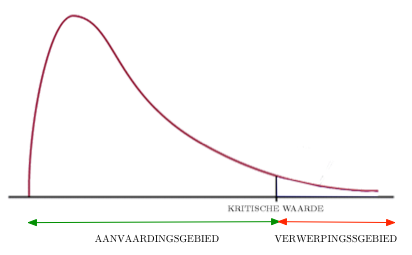
\includegraphics[width=5cm]{confidence_interval_chi_square} }}%
    \caption{Illustratie eenzijdige-toets van een ${\chi}^2$-distributie}%
    \qquad
    \subfloat{{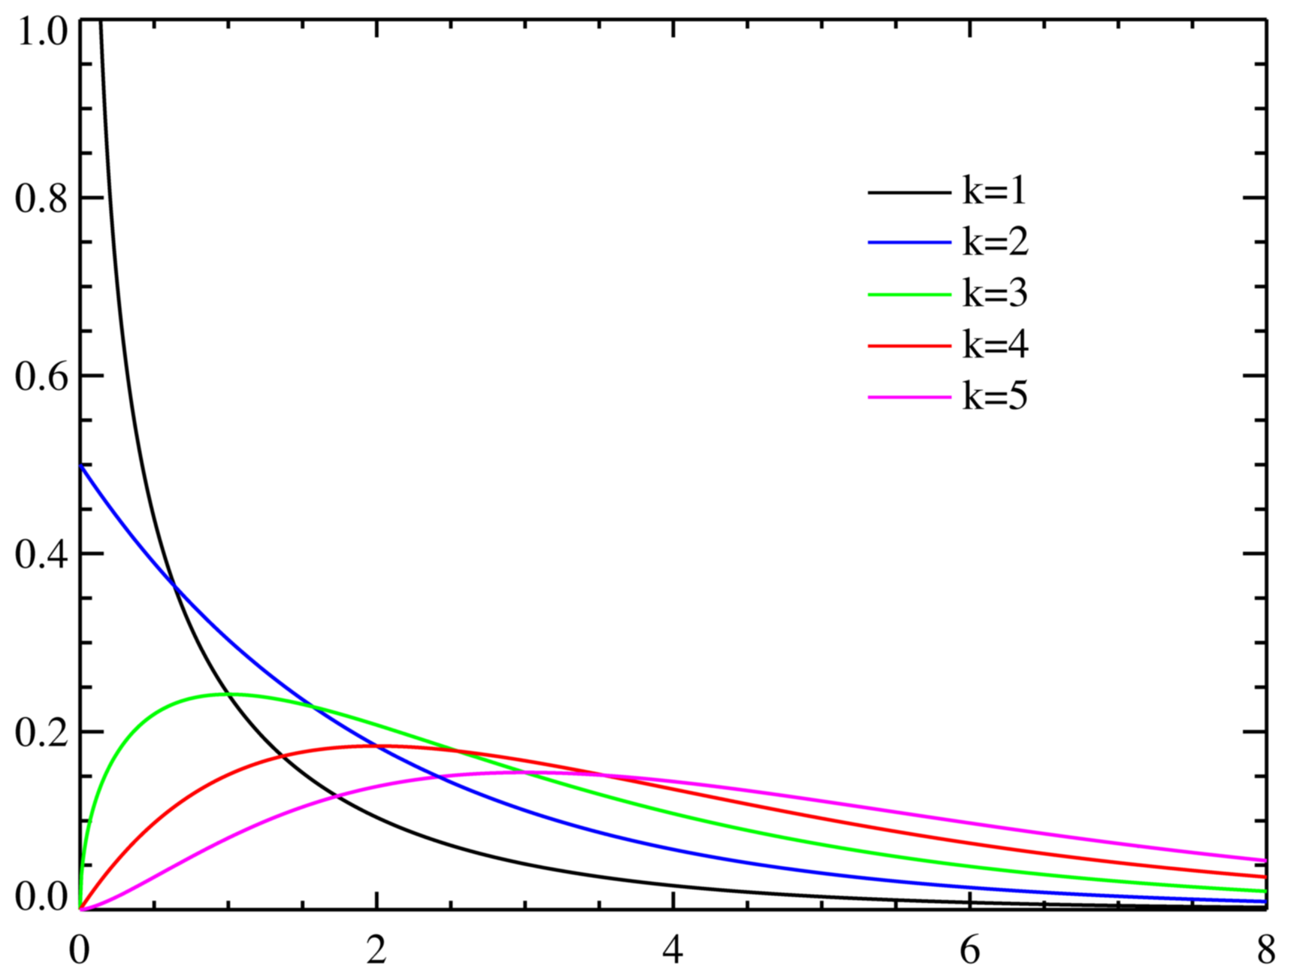
\includegraphics[width=5cm]{Chi-square_distribution} }}%
    \caption{Chi-square distributies met K vrijheidsgraden [Bron: \url{http://upload.wikimedia.org/wikipedia/commons/2/21/Chi-square_distributionPDF.png}]}%
    \label{fig:example}%
\end{figure}
%  

Kort samengevat baseert de Chi-kwadraattoets zich op de afwijking tussen de geobserveerde frequentie en de verwachte frequentie. Hoe groter het verschil, hoe waarschijnlijker men de nulhypothese kan verwerpen. En dit is waar men zich bij Bigram Collocatie gaat baseren.

\subsection{Best feature selection}\label{Low-information feature selection selection}

Als we duizende documenten verwerken, is het te voorspellen dat er enorm veel woorden algemeen voorkomen in de documenten maar niet veel informatie bijdragen over het document zelf. Het is sterk vergelijkbaar met de voorgaande techniek Bag of Words en het verwijderen van stopwoorden. Veel voorkomende features kunnen voor het document niet identificerend dienen en zorgen voor ruis op de dataset. Daarom kan men verkiezen om deze low-information features te verwijderen zodanig dat men enkel de features overhouden die echt iets zeggen over een document. Het bepalen van de informatiewinst kan gebeuren aan de hand van het aantal voorkomens in de verschillende klasses. Als een bepaalde feature voornamelijk in positieve documenten voorkomt en amper in negatieve documenten, kan men afleiden dat deze feature zeer informatief is omtrent positieve documenten. Als metriek om de informatiewinst te meten kan men wederom ${\chi}^2$ gebruiken. Chi-kwadraat laat ons namelijk toe om de correlatie tussen een bepaalde feature en de klasses te meten.
%
\subsection{Latent Semantic Analysis}\label{Latent Semantic Analysis}

Latent Semantic Analysis is een wiskundige techniek gebaseerd op statistische berekeningen. Met LSA probeert men een notie te krijgen van de semantische informatie en meer bepaald het semantisch verband tussen woorden. Bijvoorbeeld als we zoeken naar documenten met het woord ``economie'', willen we ook documenten met ``financi\"en'' terugkrijgen. Voor LSA zijn twee woorden semantisch gerelateerd als ze gebruikt worden in dezelfde context. Met het concrete voorbeeld kunnen we zeggen dat er een semantisch verband is tussen 2 woorden als ze vaak voorkomen in dezelfde documenten.
\newline
Merk op dat bij Latent Semantic Analysis het belangrijk is dat ieder woord naar \'e\'en concept verwijst.
%
\newline
Analytisch wordt LSM toegepast door \textbf{Singular Value Decomposition (SVD)} toe te passen op de terms-document matrix. SVD is een concept uit de lineaire algebra en zegt dat een matrix A opgesplitst kan worden als een product van matrixen namelijk \\
\[A = U\Sigma V^T \]
De reductie van de dimensie gebeurt aan de hand van volgend principe
%
%afbeelding van SVD in latex
\newcommand{\vect}{\mathbf}
\newcommand{\nul}{\operatorname{Nul}}
\newcommand{\col}{\operatorname{Kolommen }}
\newcommand{\row}{\operatorname{Rijen}}
\[
   A= U\Sigma V^T=
  \begin{matrix}
    \underbrace{\left[\begin{matrix}\vect u_1 & \vect u_2 & \dots & \vect u_r\end{matrix}\right.}& 
    \underbrace{\left.\begin{matrix}\vect u_{r+1} & \dots &  \vect u_m\end{matrix}\right]}\\
    \col A & \nul A^T
  \end{matrix}
  \begin{bmatrix}
      \sigma_1 & 0 & \dots & 0 & 0 & \dots & 0 \\
         0 & \sigma_2  & \dots & 0 & 0 & \dots & 0 \\
         \dots& & & & &  \\
         0 & 0 & \dots & \sigma_k  & 0 & \dots & 0 \\
         0 & 0 & \dots & 0 & 0 & \dots & 0 \\
         \dots& & & & &  \\
         0 & 0 & \dots & 0 & 0 & \dots & 0 
  \end{bmatrix}
  \begin{bmatrix}
    \vect v_1^T \\ \vect v_2^T \\ \dots \\ \vect v_r^T \\
    \vect v_{r+1}^T \\ \dots \\ \vect v_n^T
  \end{bmatrix}
  \begin{matrix}
    \left.\vphantom{\begin{bmatrix}
       \vect v_1^T \\ \vect v_2^T \\ \dots \\ \vect v_r^T 
       \end{bmatrix}}\right\}\row A \\ 
    \left.\vphantom{\begin{bmatrix}
      \vect v_{r+1}^T \\ \dots \\ \vect v_n^T 
    \end{bmatrix}}\right\}\nul A
  \end{matrix}
\] 
\newline
U is de unitaire matrix waarbij men $u_1, u_2, ... , u_n$ de linker singuliere vectors noemt. Deze stellen een document met zijn features voor. $V^T$ is de geconjugeerde getransponeerde matrix van V. $v_1, v_2, ... , v_n$ noemt men de rechter singuliere vectors en stellen de woorden met hun features over alle documenten voor. $\Sigma$ is diagonaal matrix met singuliere waarden $\sigma_1,\sigma_2,..,\sigma_n$'  op de diagonaal. De reductie van een term-document matrix naar een dimensie van $K$ gebeurt door de hoogste $K$ singuliere waarden te nemen in $\Sigma$ met de overeenkomstige singuliere vectoren uit $U$ en $V$.    
Doordat men de dimensionaliteit van de vectoren kan beperken door semantisch gelijkaardige woorden bijeen te voegen. Laat dit het toe om een soort van context groepen te cre\"eren en zo een zeker inzicht te krijgen in de dataset. Het is dan ook gebleken dat SVD toepassen een zeer nuttige eerste stap is bij text mining \cite{maas2011learning},dus ook voor ons onderzoek, omdat men nieuwe meer effici\"ente features krijgt. De nieuwe features geven meer duidelijkheid en inzicht en kunnen dienen als input voor een algoritme.


\section{Classifiers}\label{Classifiers}

\subsection{Naive Bayes Classifier}\label{Naive Bayes Classifier}

\subsection{Decision Tree}\label{Decision Tree}

\section{Valkuilen onderzoek}\label{Valkuilen onderzoek}
\subsection{Overfitting}\label{Overfitting}
\subsection{Bais}\label{Bais}
\subsection{Variantie}\label{Variantie}